\clearpage\section{Horizontal Shifts}
Now for the slightly trickier transformations. This first one is the horizontal shift, represented by the letter $h$. A horizontal shift, like a vertical one, moves the function left or right. For example, if $f(x) = x^2$, a horizontal shift one unit to the right would result in a new function $g(x) = (x - 1)^2$, where $h = 1$. 

Herein lies the confusion: If we're subtracting $x$ by $1$, why does the function move in the positive $x$ direction? Aren't negative values of $x$ on the left?

Negative values \textit{are} on the left, but it shifts to the right because the result that would've normally been produced by $f(x)$ is now produced by some larger input of $x$. 

$f(2) = 4$ because when you square $2$ you get $4$. But if you want $g(x)$ to also produce $4$, you have to use $g(3)$.
\[
    g(3) = (3 - 1)^2 = (2)^2 = 4
\]
To produce the same result, you had to input a larger value of $x$. The best example of this is getting the functions to result in $0$.
\begin{align*}
    f(0) &= (0)^2 = 0 && \text{Point at }(0, 0)\\
    g(1) &= (1 - 1)^2 = (0)^2 = 0 && \text{Point at }(1, 0)
\end{align*}
Notice that the difference for when $f(x) = g(x) = 4$ and $f(x) = g(x) = 0$, the difference in input for $f(x)$ and $g(x)$ is the value of $h$. It can then be proposed that increasing the value of $h$ to, say, $h = 3$, plugging $3$ into $h(x) = (x - 3)^2$ will produce $0$.
\[
    h(3) = (3 - 3)^2 = (0)^2 = 0 \qquad \text{Point at }(3, 0)
\]
\begin{center}
    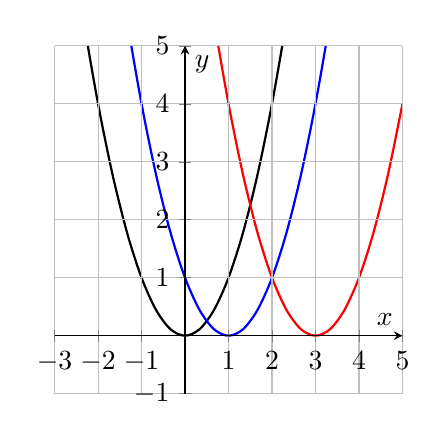
\begin{tikzpicture}
        \begin{axis} [
            axis lines=middle,
            xlabel = $x$, ylabel = {$y$},
            xmin = -3, xmax = 5,
            ymin = -1, ymax = 5,
            xtick distance={1}, ytick distance={1},
            grid = both,
            width = 6cm,
            height = 6cm,
            smooth,
            axis on top
        ]
        \addplot[black, thick, domain=-3:5] {x^2};
        \addplot[blue, thick, domain=-3:5] {(x - 1)^2};
        \addplot[red, thick, domain=-3:5] {(x - 3)^2};
        \end{axis}
    \end{tikzpicture}\\
    $f(x) = x^2$ (Black), $g(x) = (x - 1)^2$ (Blue), $h(x) = (x - 3)^2$ (Red)
\end{center}
\begin{definition}
    Given a function $f(x)$ and a horizontal shift $k$, the new function $g(x) = f(x - 1)$ is the function of $f(x)$ horizontally translated $h$ units.
    \begin{itemize}
        \item When $h < 0$, $f(x)$ moves in the negative $x$ direction (left).
        \item When $h > 0$, $f(x)$ moves in the positive $x$ direction (right).
        \item When $h = 0$, $f(x) = g(x)$. The function does not move.
    \end{itemize}
\end{definition}